\documentclass[12pt, letterpaper, a4paper]{article}
\usepackage{graphicx}
\usepackage{textcomp}
\usepackage[hungarian]{babel}
\usepackage[T1]{fontenc}
\usepackage[utf8]{inputenc}
\usepackage{caption}
\usepackage{subcaption}
\usepackage{csquotes}
\graphicspath{{./images/}}
\usepackage[
    style=ieee,
  ]{biblatex}
\addbibresource{soc.bib}

\usepackage{listings}
\usepackage[svgnames]{xcolor}
\usepackage{tikz}
\usetikzlibrary{shapes.geometric, arrows, calc}

\definecolor{dkgreen}{rgb}{0,0.6,0}
\definecolor{gray}{rgb}{0.5,0.5,0.5}
\definecolor{mauve}{rgb}{0.58,0,0.82}

\lstset{frame=tb,
  language=Bash,
  aboveskip=3mm,
  belowskip=3mm,
  showstringspaces=false,
  columns=flexible,
  basicstyle={\small\ttfamily},
  numbers=none,
  numberstyle=\tiny\color{gray},
  keywordstyle=\color{blue},
  commentstyle=\color{dkgreen},
  stringstyle=\color{mauve},
  breaklines=true,
  breakatwhitespace=true,
  tabsize=2
}

\tikzstyle{box} = [rectangle, rounded corners, minimum width=3cm, minimum height=0.5cm,text centered, draw=black, fill=red!30]
\tikzstyle{arrow} = [thick,->,>=stealth]


\title{\textcolor{RoyalBlue}{\textbf{Heterogén SoC rendszerek házi feladat}}}
\author{\textcolor{RoyalBlue}{Batcher Odd-Even-Merge algoritumus skalár megvalósítás} \\ \\ Nyiri Levente}
\date{2025 Október}
\begin{document}
\selectlanguage{hungarian}
\maketitle

\newpage

\section{Algoritmus}

Batcher Odd-Even-Merge algoritmusa úgy műdödik, hogy elfelezzük a listánkat, külön-külön rendezzük a feleket, majd a páros és páratlan indexű elemeket is összehasonlítjuk. Ezután már csak egyszer kell a szomszédos elemeket összehasonlítani és a számhalmunk rendezve van.

Ez egy rekurzív algoritmus. Két részből áll: egy olyan algoritmus ami a két rendezett felet kialakítja (sort), és egy olyan ami ezeket a rendezett feleket felhasználva rendez tovább (merge).

\subsection{sort}

A tömbünk hosszát elosztjuk 2-vel, \( m = \frac{lenght}{2} \), majd ezt átadva hosszként újra meghívjuk a függvényt. Ismét meghívjuk afüggvényt, ezúttal a kezdeti pontot \(m\)-el eltolva. Végül meghívjuk a merge függvényt, ami abban az esetben ha csak két elemet adunk át, akkor összehasonlítja és szükség esetén megcseréli őket. Hosszabb lista esetén ő is rekurzívan működik, először meghívja önmagát 0-ás indextől kezdve, majd ismét, 1-es indextől. A következő lépése, hogy összehasonlítsa az átadott lista páratlan indexű elemeit.
%TODO: ezt átírni kevésbé katyvaszosra

A működést legjobban rekurzív algoritmusoknál szerintem call stack-el lehet szemléltetni, ez látható a \ref{fig:call-stack}.-ik ábrán.

\newpage

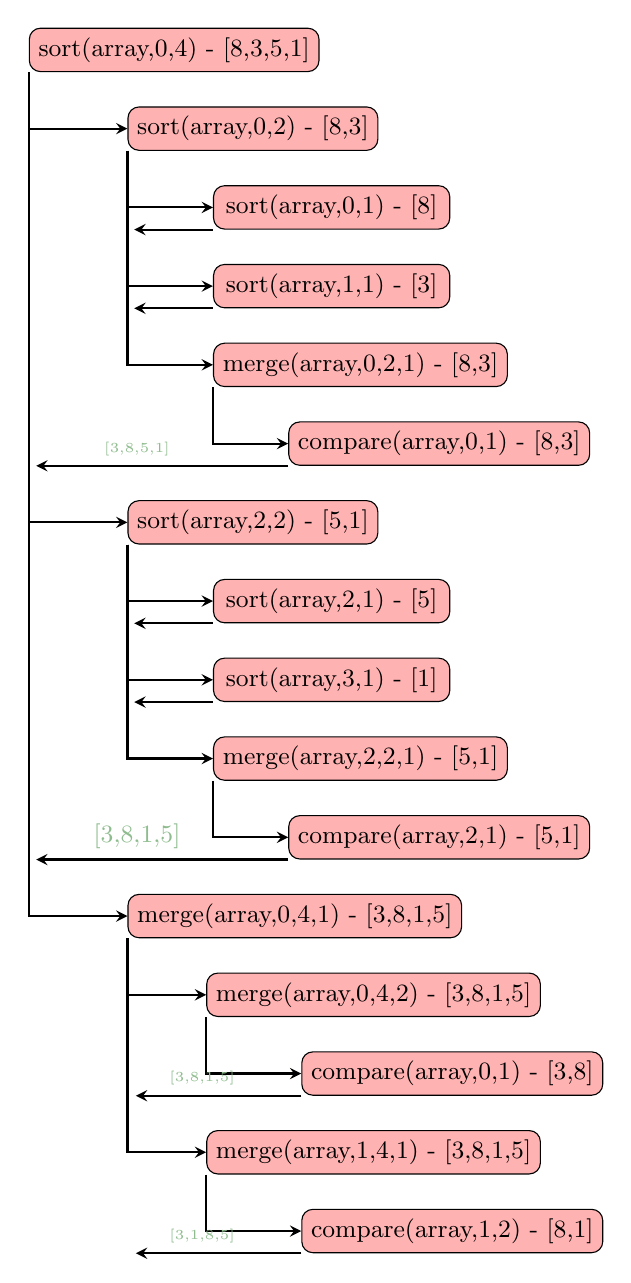
\begin{tikzpicture}[node distance=1cm, font=\small]
  \node (1) [box] {sort(array,0,4) - [8,3,5,1]};

  \node (2) [box, below of=1, xshift=1cm] {sort(array,0,2) - [8,3]};

  \node (3) [box, below of=2, xshift=1cm] {sort(array,0,1) - [8]};
  
  \node (4) [box, below of=3, xshift=0cm] {sort(array,1,1) - [3]};
  
  \node (5) [box, below of=4, anchor=west] at (4.west) {merge(array,0,2,1) - [8,3]};
  \node (6) [box, below of=5, xshift=1cm] {compare(array,0,1) - [8,3]};
  \node (7) [box, anchor=west] at ($(2.west) + (0,-5)$) {sort(array,2,2) - [5,1]};
  \node (8) [box, below of=7, xshift=1cm] {sort(array,2,1) - [5]};
  \node (9) [box, below of=8, xshift=0cm] {sort(array,3,1) - [1]};
  \node (10) [box, below of=9, anchor=west] at (9.west) {merge(array,2,2,1) - [5,1]};
  \node (11) [box, below of=10, xshift=1cm] {compare(array,2,1) - [5,1]};
  \node (12) [box, anchor=west] at ($(7.west) + (0,-5)$) {merge(array,0,4,1) - [3,8,1,5]};
  \node (13) [box, below of=12, xshift=1cm] {merge(array,0,4,2) - [3,8,1,5]};
  \node (14) [box, below of=13, xshift=1cm] {compare(array,0,1) - [3,8]};
  \node (15) [box, anchor=west] at ($(13.west) + (0,-2)$) {merge(array,1,4,1) - [3,8,1,5]};
  \node (16) [box, below of=15, xshift=1cm] {compare(array,1,2) - [8,1]};


  \draw [arrow] (1.south west) |- (2);
  \draw [arrow] (2.south west) |- (3);
  \draw [arrow] (2.south west) |- (4);
  \draw [arrow] (2.south west) |- (5);
  \draw [arrow] (5.south west) |- (6);
  \draw [arrow] (1.south west) |- (7);
  \draw [arrow] (7.south west) |- (8);
  \draw [arrow] (7.south west) |- (9);
  \draw [arrow] (7.south west) |- (10);
  \draw [arrow] (10.south west) |- (11);
  \draw [arrow] (1.south west) |- (12);
  \draw [arrow] (12.south west) |- (13);
  \draw [arrow] (13.south west) |- (14);
  \draw [arrow] (12.south west) |- (15);
  \draw [arrow] (15.south west) |- (16);
  \draw [arrow] (3.south west) |- ++(-1,0);
  \draw [arrow] (4.south west) |- ++(-1,0);
  \draw [arrow] (6.south west) |- node[pos=0.8, above] {\tiny{\color{DarkSeaGreen}{[3,8,5,1]}}} ++(-3.2,0);
  \draw [arrow] (8.south west) |- ++(-1,0);
  \draw [arrow] (9.south west) |- ++(-1,0);
  \draw [arrow] (11.south west) |- node[pos=0.8, above] {\color{DarkSeaGreen}{[3,8,1,5]}} ++(-3.2,0);
  \draw [arrow] (14.south west) |- node[pos=0.8, above] {\tiny{\color{DarkSeaGreen}{[3,8,1,5]}}} ++(-2.1,0);
  \draw [arrow] (16.south west) |- node[pos=0.8, above] {\tiny{\color{DarkSeaGreen}{[3,1,8,5]}}} ++(-2.1,0);
\end{tikzpicture}


\end{document}
